% !TEX TS-program = pdflatex
% !TEX encoding = UTF-8 Unicode
% !TEX ROOT = main.tex

\newcounter{zahl}
% \newcommand{\altstadtkarte}{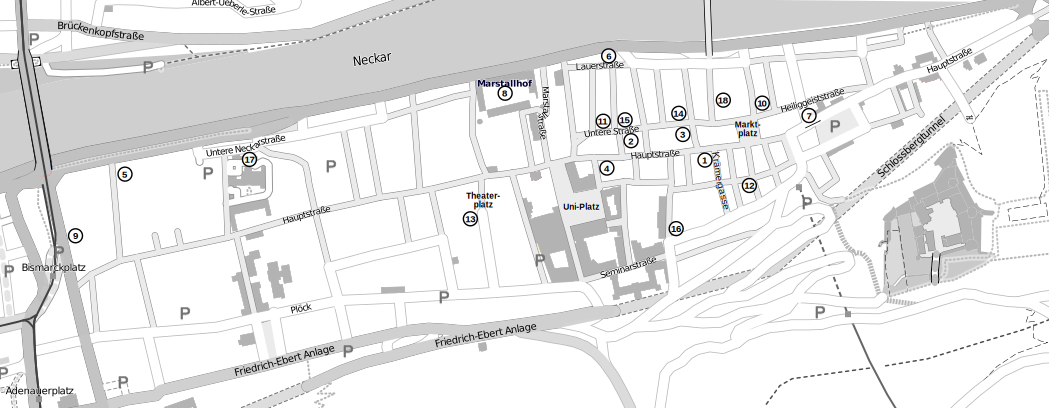
\includegraphics[width=\textwidth, trim=10mm 0mm 80mm 0mm, clip]{media/altstadtkarte}} % Vektorgrafik einbinden
\newcommand{\place}[4]{\item[(\stepcounter{zahl}\thezahl) #1](#2)\\ #3\\\emph{Preis:} #4}

\section{Bars, Kneipen \& Clubs}
Preis: $\star$ teuer, $\star\ \star$ noch teurer, $\star\ \star\ \star$ extrem teuer


\begin{description}

%    \place{Alfredo}{Untere Straße}{Wirklich sehr leckere Pizza, der Chef sorgt für den echt italienischen Flair.}{$\star$}

%    \place{Cave 54}{Krämergasse 1}{(Deutschlands ältester) Jazzkeller. Kostet am Wochen\-ende Eintritt, hat dafür allerdings noch nach 3 Uhr geöffnet.}{$\star\ \star$}

%    \place{Coyote}{Hauptstraße}{Einer der Orte, um eine Kneipentour durch die Altstadt starten zu lassen. Weizenbier, Cocktails und Shots sind brauchbar und brauchen nicht ewig.}{$\star\ \star$}

    \place{Destille}{Untere Straße 16}{Große Auswahl an Shots. Kultladen mit ständig wechselnder Dekoration.}{$\star\ \star$}

%    \place{Eckstein}{am Fischmarkt 3}{Abgefahrene Kneipe. Je nach Wochentag ändert sich das Programm. Es gibt jedoch immer einen Kicker und reichlich Platz. Drei Mal wöchentlich Zaubershows.}{$\star\ \star$}

%    \place{Hard Rock Cafe}{Hauptstraße 142}{Montags Bier für \EUR{1}, ab 18 Uhr Cocktails für \EUR{4}. Musik wie man es erwartet, durchgehend Rock.}{$\star$}

%    \place{Havanna}{Neckarstaden 24}{Cocktailbar mit Möglichkeit zum Salsa tanzen.}{$\star\ \star\ \star$}

    \place{Hemingway's}{Fahrtgasse 1}{Hier kann man wunderbar den Neckar beobachten. Innenbereich urig, aber nicht für größere Gruppen geeignet. Nachmittags und Abends sollte man auch für draußen vorher anrufen und reservieren. \url{www.hemingways-heidelberg.de}}{$\star\ \star$}

    \place{Karl}{Lauerstraße 7-9}{Raucherkneipe mit Billardtisch und Dartscheibe. Gut, um bei 'nem exzessiven Bierabend zu versacken. Hard Rock und Metal, Lautstärke gnadenlos. Regelmäßig Live-Konzerte. \url{http://www.k-a-r-l.de}}{$\star\ \star$}

%    \place{Karlstorbahnhof}{Am Karlstor\,/\,S-Bahnhof Altstadt}{Richtig gute Diskothek (Nicht nur; im Gebäude gibts auch Theater, Lesungen etc. -- viel Kultur) mit sehr variabler Musik. Was zum Tanzen und weniger zum Trinken, denn die Preise können sich meistens sehen lassen, genauso der Eintritt.}{$\star\ \star\ \star$}

    \place{Marstall}{Marstallhof}{Unimensa und -caf\'e in historischem Gebäude mit Biergarten im Innenhof. Mensapreise! Gut geeignet zum Vorglühen in der Altstadt.}{$\star$}

%    \place{Maxbar}{Marktplatz 5}{Hier gibt es des öfteren Live-Musik}{$\star\ \star$}

%    \place{Medoc}{Bismarckplatz}{Cafe Restaurant, das für ca. \EUR{5} wechselnde Mittagsgerichte anbietet. Man kann draußen sitzen und den Betrieb auf dem Bismarckplatz beobachten.}{$\star\ \star$}

    \place{Mel's}{Heiliggeiststr. 1}{Gewölbekeller, meist Rock und Pop, Tanzfläche. Spät abends sehr voll. Donnerstags \glqq{}Happy \emph{Thirst}\/day\grqq{} (alle einfachen Longdrinks \EUR{2}) und jeden Tag Happy Hour bis 23 Uhr.\\\url{www.jinx-heidelberg.de/mels}}{$\star\ \star$} % Obwohl man hier nicht vorher reservieren kann, habe ich trotzdem die URL angehängt, weil das Leute, die danach suchen, sonst vielleicht nicht gleich kapieren (siehe URL).

    \place{Mohr}{Untere Straße}{Hoher MedizinerInnen-Anteil, Einlass erst ab 20 Jahren und spät abends gerammelt voll. Drinnen wird dafür allerdings auf den Tischen getanzt.}{$\star\ \star$}

%    \place{Orange}{Ingrimmstraße 26a}{Eine Kneipe wie ein Wohnzimmer. Eng, aber gemütlich. Bietet sehr leckeres Bier aus Tschechien an, ist aber leider eher verraucht. Es gibt sogar Brettspiele.}{$\star\ \star$}

%    \place{Palmbräugasse}{Untere Straße}{Hier gibts das selbstgebraute Palmbräu. Palmen gehören zwar nicht typisch zu Heidelberg, aber die Schnitzel in der Palmbräugasse.}{$\star\ \star$}

%    \place{Regie}{Theaterplatz}{Riesenauswahl an Cocktails, die nach Filmen benannt und meist recht schick dekoriert sind. Cooles Specials- und Aktionensystem und leckere Flammkuchen}{$\star\ \star\ \star$}

    \place{Reichsapfel}{Untere Straße}{Sehr geräumig. Moderner Vorderbereich und urigere Atmosphäre im hinteren Teil, welcher über den Innenhof zugänglich ist. Dort findet man oft Platz, wenn sonst alles voll ist.}{$\star\ \star$}

%    \place{Sonderbar}{Untere Straße}{Jede Menge Absinth, auch viel guten Rum und Whisky. Musik Hard \& Heavy. Keine Angst vor dem Wirt! Oft sehr voll. Raucherkneipe.}{$\star\ \star$}

%    \place{Tangente}{Kettengasse 23}{Hoher JuristInnenanteil und teils ältere Menschen. Türsteher und Gesichtskontrolle, dafür aber kein Eintritt. Hier kann man bis in die frühen Morgenstunden tanzen, man sollte allerdings keine Platzangst haben.}{$\star\ \star$}

    \place{Dubliner}{Hauptstraße 93}{Großer Irish Pub. Donnerstags Pubquiz oben ab 21 Uhr, freitags ab 22 Uhr Karaoke.}{$\star\ \star$}

    \place{Vater Rhein}{Untere Neckarstraße 20}{Legendär für seine \EUR{1,90}-Spaghetti zum Getränk bis kurz vor 2 Uhr nachts. Großer Nichtraucherbereich. \emph{Die} Studikneipe in Heidelberg. Tagungsort des Heidelberger ZaPF-Stammtisches. Hier lässt sich der Abend gemütlich ausklingen. Geöffnet ab 20 Uhr. Donnerstag bis Samstag abends immer voll. Große Gruppen sollten einen Tag vorher reservieren. Tel.: 06221\,21371}{$\star$}

    \place{Vetter}{Steingasse 9}{Kleine Brauerei, Heidelberger Spezialität. Urig, Maßbier To Go gibts da für \EUR{3} plus Pfand und schmeckt hervorragend. Ansonsten gutbürgerliche Küche und überwiegend ältere Klientel.}{$\star\ \star$}

\end{description}

% trim=l b r t
\hspace*{-6mm}
% \altstadtkarte
  \todo{altstadtkarte aus media/altstadtkarte.svg einbinden}
    \todo{Boho vllt noch einfügen}

%%%%%%%%%
\begin{description}

%    \place{Bar 133}{Wohnheim INF 133}{Wohnheimsbar, eigentlich nur für Bewohner der 1xx Wohnheime. Mittwochs und sonntags geöffnet mit gutem Angebot, günstigen Cocktails und Tischkicker. Immer wieder für einen Absturz gut.}{$\star$}

%	\place{Comabar}{Comenius-Haus}{Bar des Comenius-Hauses direkt am Bunsengymnasium. Dienstags und Donnerstags geöffnet, super Team, günstige Cocktails, Kicker und Tischtennisplatte vorhanden. Definitiv empfehlenswert.}{$\star$}

%    \place{Breidenbach Studios}{Hebelstraße 18}{Absoluter Hipster-Laden: Ehemalige Gasflaschenhandlung, die zu einem Künstlerhaus und Coworking-Space umgebaut wurde. Hier finden immer wieder großartige Partys statt.}{$\star\ \star\ \star$}

    \place{Halle 02}{Bahnstadt}{Rock- Mainstream- und Electroparties. Viel Platz und am Wochenende voll. Am Donnerstag während der ZaPF spielt hier Schandmaul live.}{$\star\ \star$}

%    \place{O'Reilly's}{Brückenkopfstraße 1}{Irish Pub mit Karaoke. Größere Gruppen sollten vorher anrufen! \url{www.oreillys.com/heidelberg}}{$\star\ \star\ \star$}

    \place{Villa Nachttanz}{Im Klingenbühl 6}{Alternativer Kulturverein -- rechnet mit allem außer Mainstream. Sehr günstig, mit Lagerfeuer im Garten. Lohnt sich jedes Mal.}{$\star$}

\end{description}
